\documentclass[tikz]{standalone}
\usepackage{tikz}

\tikzset{
    ->, 
    level distance = 12em,
    minimum size=2em,
    %edge from parent/.style={draw,thick},
    level 1/.style={sibling distance=6em},
    level 2/.style={sibling distance=3em},
    thick/.style = {line width=1.5pt},
    extra thick/.style = {line width=3.5pt},
    red node/.style={shape=circle,draw=red,fill=red!40,thick,inner sep=1.2},
    blue node/.style={shape=circle,draw=blue,fill=blue!40,thick,inner sep=1.2}
}

\tikzstyle{round}=[thick,draw=black,circle]

\begin{document}

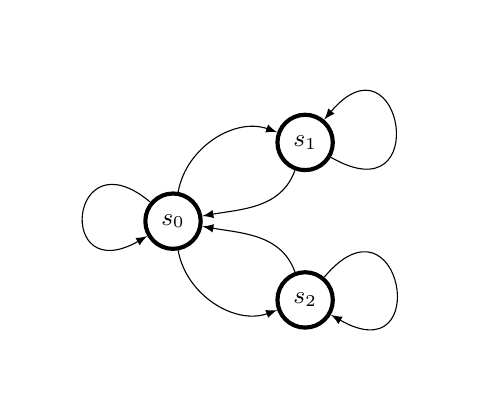
\begin{tikzpicture}[auto,node distance=8mm,>=latex,font=\small]
    \tikzstyle{round}=[thick,draw=black,circle]
    \node[round] (s0) {$s_0$};
    \node[round, above=10mm, right=13mm] (s1) {$s_1$};
    \node[round, below=10mm, right=13mm] (s2) {$s_2$};

    \draw[->] (s0) [out=80,in=160] to node {} node [swap] {} (s1);
    \draw[->] (s0) [out=-80,in=200] to node {} node [swap] {} (s2);
    \draw[->] (s1) [out=250,in=10] to node {} node [swap] {} (s0);
    \draw[->] (s2) [out=110,in=-10] to node {} node [swap] {} (s0);

    \draw[->] (s0) [out=140,in=210,loop] to node {} node [swap] {} (s0);
    \draw[->] (s1) [out=-30,in=50,loop] to node {} node [swap] {} (s1);
    \draw[->] (s2) [out=50,in=-30,loop] to node {} node [swap] {} (s2);


\end{tikzpicture}

\end{document}
